\documentclass[12pt]{article}

\usepackage{comptype}

\title{%%
Lista de Computação para Arquitetura\\
{\normalsize LAMO / FAU / UFRJ}
}

\author{%%
Pedro Maciel Xavier \\ 
\texttt{pedromxavier@poli.ufrj.br}
}

\begin{document}
	\maketitle
	\section*{Introdução}
	
	Essa lista de exercícios está sendo pensada para uma disciplina de Computação no curso de Arquitetura e Urbanismo.
	
	\cc
	
	%% \tableofcontents
	
	\problemsec[0]{Intersecção de Retângulos}
	
	Uma maneira simples de representar retângulos em um computador é através de um par de pontos, onde cada ponto é um par ordenado $(x, y)$. Por convenção, o primeiro ponto indica o canto superior esquerdo do retângulo; e o segundo, o canto inferior direito.\\
	
	%% \begin{figure}[H]
	\centering
	\begin{tikzpicture}
	\draw[draw=black] (11.1,5.5) rectangle ++(0.3,0.3);
	\end{tikzpicture}
\end{figure}
	
	Assim, o retângulo \textcolor{blue}{\textbf{azul}} pode ser descrito pelos pares $(1, 4)$ e $(5, 2)$, enquanto o retângulo \textcolor{red}{\textbf{vermelho}} é dado pelos pontos $(3, 3)$ e $(6, 1)$. A intersecção entre os dois é justamente a área \textcolor{indigo}{\textbf{lilás}} que se encontra entre os pontos $(3, 3)$ e $(5, 2)$. \\
	
	\quest Fazer uma função que, dados dois retângulos, retorna a intersecção entre eles, ou seja, um outro retângulo ou \stmt{None}, caso não haja sobreposição.\\
	
	\example
	\begin{lstlisting}
>>> A = (1, 4, 5, 2)
>>> B = (3, 3, 6, 1)
>>> C = intersec(A, B)
>>> print(C)
(3, 3, 5, 2)
	\end{lstlisting}
	
	\pagebreak
	
	\problemsec[0]{Anos bissextos}
	
	A humanidade sempre teve problemas com a contagem dos anos, uma vez que estes duram 365,24 dias. O calendário Juliano, que vigorou de 45 a.C. até 1582 d.C., introduziu o uso dos anos bissextos acrescentou um dia a cada 3 anos. O erro só foi percebido décadas depois e o acréscimo foi abandonado. Isso fez com que se acumulasse um erro de cerca de 10 dias até o momento da transição para o calendário Gregoriano. Por conta disso, os dias entre 4 e 15 de outubro de 1582 simplesmente não existiram.\\
	
	Com este novo calendário foi definida a nova regra para o cálculo dos anos bissextos:
	
	\begin{itemize}
		\item De 4 em 4 anos é ano bissexto.
		\item De 100 em 100 anos não é ano bissexto.
		\item De 400 em 400 anos é ano bissexto.
		\item Prevalecem as últimas regras sobre as primeiras.
	\end{itemize}
	
	\quest Sabendo que o ano 2000 foi bissexto, crie uma função que, dado um ano, informe se ele é bissexto ou não, retornando \stmt{True} ou \stmt{False}, respectivamente.\\
	
	\example
	\begin{lstlisting}
	>>> bissexto(2000)
	True
	>>> bissexto(2100)
	False
	>>> bissexto(2104)
	True
	\end{lstlisting}
	
	\pagebreak
	
	\problemsec[0]{Coordenadas polares.}
	
	Estamos acostumados a pensar em coordenadas cartesianas na hora de descrever a geometria de um determinado objeto. No entanto, o sistema de coordenadas deve ser escolhido conforme o cenário em que se está trabalhando.
	
	\begin{figure}[H]
	\centering
	\resizebox{200pt}{!}{%
	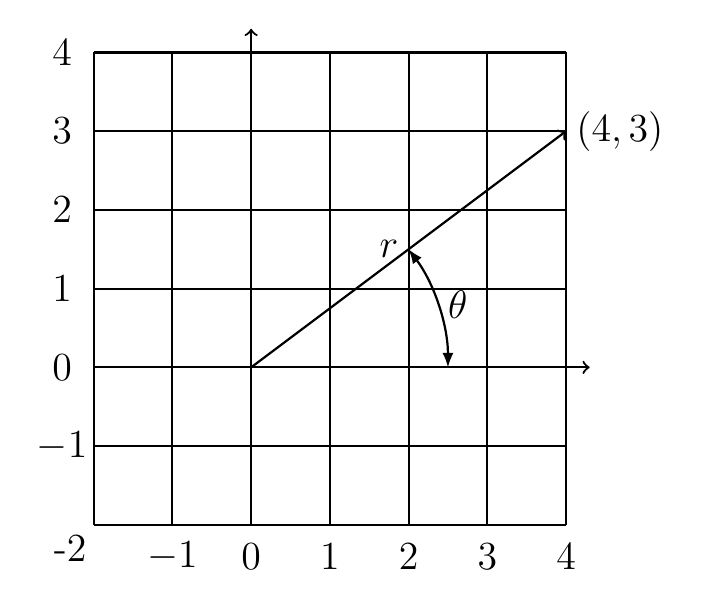
\begin{tikzpicture}[thick,font=\Large]
		\draw[step=1.0,black,thick] (-2,-2) grid (4, 4);
		\foreach \i in {-1, ..., 4} {
			\node[align=left] at (\i, -2.4) {$\i$};
			\node[align=left] at (-2.4, \i) {$\i$};
		}
		\node at (-2.3, -2.3) {-2};
		%% Axis
		\draw[->] (4, 0) -- (4.3, 0);
		\draw[->] (0, 4) -- (0, 4.3);
		%% else
		\draw[thick, ->] (0, 0) -- (4, 3) node [midway, left] {$r$} node [right] {$(4, 3)$};
		\draw[latex-latex]  (0:2.5) arc (0:36.87:2.5) node[midway, right]{$\theta$};
	\end{tikzpicture}
	}
	\caption{Coordenadas cartesianas e polares.}
\end{figure}
	
	O ponto $(4, 3)$, quando escrito em coordenadas polares, nos dá:
	\begin{align*}
		r &= \sqrt{4^2 + 3^2} = \sqrt{16 + 9} = \sqrt{25} = 5\\
		\theta &= \arctan\frac{3}{4} = 0.01123 \text{ rad} \approx 36.87^{\circ}
	\end{align*}
	
	\quest Construa duas funções: \texttt{polar(x, y)} levará um ponto em coordenadas cartesianas $(x, y)$ para a forma polar $(r, \theta)$ e \texttt{cart(r, theta)}, que fará o caminho contrário.\\
	
	\example
	\begin{lstlisting}
>>> polar(-1, 0)
(1, 3.141592653589793)
>>> cart(2, math.pi)
(-2, 0)
	\end{lstlisting}
	
	\pagebreak
	
	\problemsec[0]{Sequência de \emph{Collatz}}
	
	A sequência de \emph{Collatz} é obtida aplicando sucessivamente a função
	{\large
	\begin{align*}
		f(n) = \begin{cases}
		3n + 1, &\text{ se } n \text{ for ímpar}\\
		n \div 2, &\text{ se } n \text{ for par}
		\end{cases}
	\end{align*}
	}
	Por exemplo, começamos com $n = 26$. Após sucessivas aplicações temos:
		$$26 \to 13 \to 40 \to 20 \to 10 \to 5 \to 16 \to 8 \to 4 \to 2 \to 1$$
	Isso nos dá uma sequência com $11$ números. $40$ é maior que $26$, mas sua sequência só teria $9$ números.\\
	\\
	Ainda não se sabe se todos os números induzem uma sequência que termina em $1$. No entanto, até agora não foi encontrado um número sequer em que isso não tenha acontecido!\\
	\\
	\quest Faça uma função que calcule o comprimento da sequência gerada a partir de um número natural $n$ qualquer.\\

	\example
	\begin{lstlisting}
>>> collatz(26)
11
>>> collatz(40)
9
>>> collatz(1)
1
	\end{lstlisting}
	
\end{document}